\documentclass[english,titlepage]{article}
%\documentclass[12pt,a4paper,titlepage]{article}
\usepackage{mathpazo}
\usepackage[T1]{fontenc}
%\usepackage[utf8]{inputenc}
\usepackage[a4paper]{geometry}
\geometry{verbose,tmargin=3cm,bmargin=3cm,lmargin=2.5cm,rmargin=2.5cm}
\pagestyle{plain}
\usepackage{authblk}


\usepackage{babel}

\usepackage{float}
\usepackage{textcomp}
\usepackage{amstext}
\usepackage{graphicx}
\usepackage{setspace}
\usepackage[authoryear]{natbib}
%\usepackage{cite}
\author[1]{Rebecca B Harris}
\author[2]{Christina Ewers-Saucedo}
\author[3]{Lucy Li}
\author[4,5,6]{Julia A Palacios}
\author[7]{George Shirreff}
\affil[1]{Department of Biology, University of Washington, Seattle, WA 98122}
\affil[2]{University of California at Davis, Davis, CA}
\affil[3,7]{Department of Infectious Disease, Imperial College London, London, UK}
\affil[4]{Department of Organismic and Evolutionary Biology, Harvard University, Cambridge, MA, 02138}
\affil[5]{Center for Computational Molecular Biology, Brown University, Providence, RI 02912}
\affil[6]{Department of Ecology and Evolutionary Biology, Brown University, Providence, RI 02912}
%\usepackage[square,sort,comma]{natbib}
\date{}
\title{multiNe: the many facets of effective population size.}
\begin{document}
\bibliographystyle{molecol.bst}

\maketitle

\section{Abstract}
Inference of effective population size trajectories over time from genomic data is very useful in areas such as conservation biology and surveillance of infectious diseases. It allows us to gain insight about the past evolutionary dynamics from present-day genomic data. [Something about different methods and sources of data to estimate the same thing and the motivation of this package] 
\section{Introduction}

The effective population size trajectory over time ($N_e(t)$) is a key parameter in understanding the evolutionary dynamics of a population. Wright (1931) formally described $N_e(t)$ as the number of breeding individuals in an ideal population that show the same rate of genetic drift as the population being studied \citep{Wright1931}. Since then, it has become the primary parameter of concern for evolution, ecology, conservation biology studies and surveillance of infectious diseases. Estimates of $N_e$ encompass the effects of both demographic and genetic processes in finite populations, thus effectively quantifying the rate and timing of molecular evolution \citep{Caballero1994}. 

Despite its wide popularity, the calculation of $N_e$ in natural populations remains challenging and multiple methods have been developed to estimate $N_e$ indirectly from genetic data. Here, we distinguish between two fundamentally different ways to estimate $N_e$...


On the one hand, coalescent theory provides a means to estimate Ne over evolutionary times using either summary statistics, such as the number of segregating sites \cite{Watterson1975}, number of alleles (Ewens 1972), heterozygosity \citep{Kimmel1998}, variance of the number of microsatellite repeats \citep{Kimmel1998}, or using the shape of the genealogy itself \citep{Kingman1982}. The parameter calculated is theta, the mutation-rate scaled effective population size. Knowing the mutation rate allows us then to convert theta into $N_e$. Several of these theta calculators are available in the R package pegas \citep{Paradis2010}. 

\section*{Functionality}
\subsection*{Phy2Sky}

Coalescent theory states that the rate at which the lineages in a genealogy coalesce is inversely proportional to the effective population size \citep{slatkin_pairwise_1991}. This relationship allows the estimation of changes in $N_e(t)$ over time to be based on changes in the coalescent pattern of the genealogy, which can be visualized in skyline plots. Here, we extend the coalescent method implemented in the \texttt{R} package \texttt{ape} \citep{Paradis2004} by allowing for genealogies with heterochronous dated tips. This will be of particular value in epidemiological studies where there is precise information about the sample collection time.


The \texttt{Phy2Sky} function takes as its first argument a \texttt{multiPhylo} object, the typical output of widely used Bayesian phylogenetic programs. We provide a function, \texttt{burninfrac}, to discard a user-defined proportion of the raw posterior distribution as burn-in. Given a set of trees, \texttt{Phy2Sky} will output the end times and $N_e(t)$ estimates of each coalescent interval for each tree. Alternatively, results from multiple trees can be merged and \texttt{Phy2Sky} will generate a table with all possible events across all trees. Users may then plot the median $N_e(t)$ skyline with the 95\% confidence intervals.

Branch-lengths can be converted from substitutions per site to time units by defining the clock rate in the scaling option of \texttt{Phy2Sky}. Certain users may want to fix the skyline to reflect specific sampling dates. We provide the tools to extract sampling dates from tip names and use these in the skyline output plot.

Skyline data are usually presented by a step function, consisting of only vertical and horizontal lines, implying that for a given period the best estimate for the effective population size is a certain value. We provide numerous functions to manipulate the plotting of these stepwise graphs. For some analyses, it may be preferred that points on the graph are joined by straight sloping lines, implying that the effective population size during this period changes in a regular fashion. We also allow users to combine neighbouring time intervals until a minimum time interval cutoff is met. [Fig \#? Have figure to show these types of graphs?] 
On the other hand, Ne can be estimated by observing and quantifying deviations from exceptions of infinitely large populations. 
  
\subsection*{Inferring Ne from multiple genealogies} 
In the era of next-generation sequencing, data from multiple effectively unlinked genetic loci are rapidly becoming the norm. Evolutionary dynamics of such independently evolving loci are governed by the same demographic history of the population under study, enabling straightforward estimation of effective
population size trajectories based on multilocus genetic data. Increasing the number of loci improves precision of the  estimation of effective population size trajectories, which is critical for nonparametric procedures that often suffer from large Bayesian Credible Intervals (BCIs). Here, we implement a method to infer effective population size trajectories ($N_{e}$) from multiple independent genealogies using integrated nested Laplace approximation (INLA) under the coalescent model. Here, we assume that our data consist of $n$ independent genealogies $g_{1},\ldots,g_{n}$ and we are interested in estimating $N_{e}(t)$. Following \citet{palacios2012INLA}, we model $\log N_{e}(t)$ as a log Brownian motion process with precision parameter $\tau$, that is, $\log N_{e}(t) \sim BM(\tau)$. Our approach infers $N_{e}(t_{i})$ at $t_{1},\ldots,t_{B}$ regularly spaced time points. Our point estimates correspond to posterior marginal medians at each time point and our credible regions correspond to 95\% Bayesian Credible Intervals (BCIs). Posterior marginals are approximated using \texttt{R-INLA} \citep{INLA_2009} . Our implementation extends the method implemented in \texttt{R-phylodyn} to account for multiple independent genealogies.
\begin{figure}
\begin{center}
      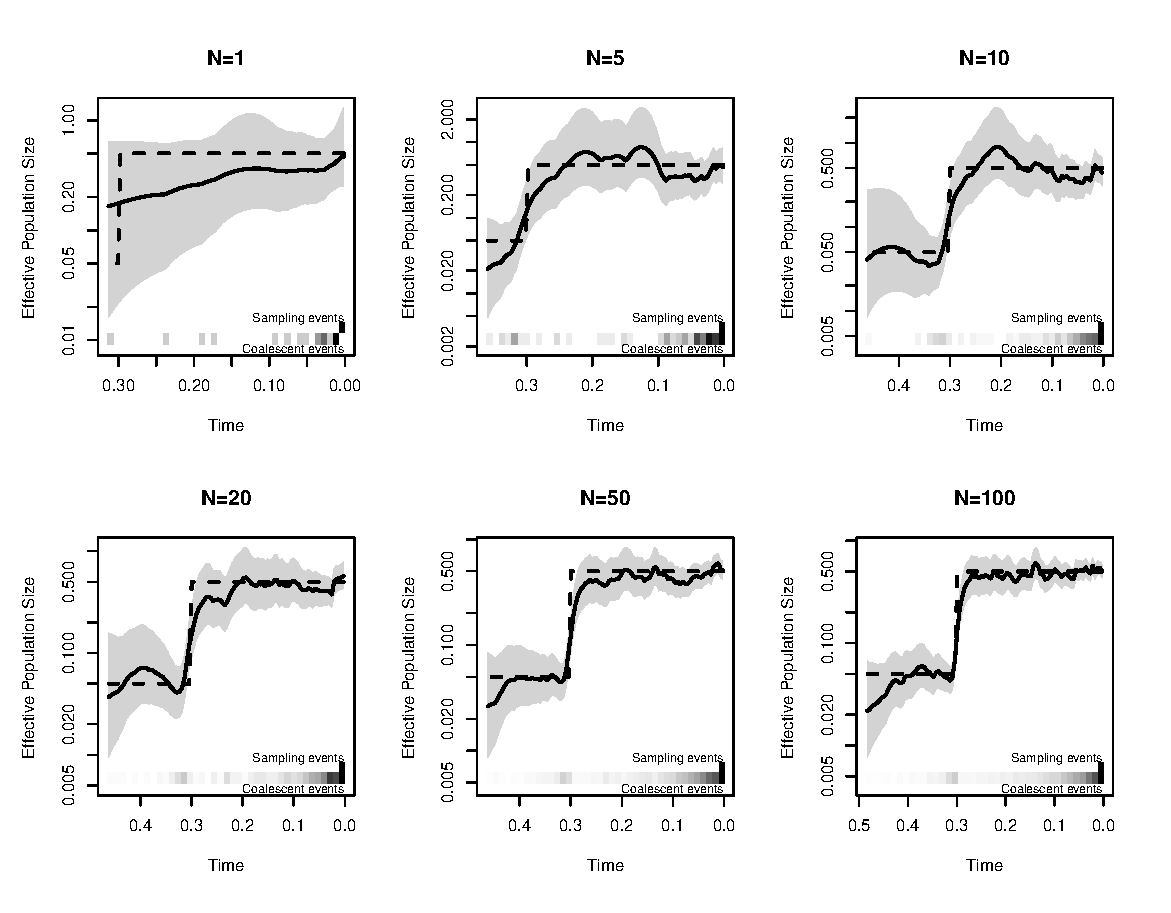
\includegraphics[scale=0.8]{Figures/Bottle_20_independent.eps}    \end{center}
      \caption{\small{INLA-based inference of $N_{e}(t)$ from $N=1$ to $N=100$ independent genealogies simulated under a population bottleneck (dashed line). Posterior median is represented by a solid black line and 95\% BCIs are represented by the shaded areas. Increasing the number of independent genealogies improves inference.}}

\end{figure}
 
%\subsection*{Inferring Ne from sequential local genealogies}
%This is the SMC implementation.
% I decided not to include this code in this package


\subsection*{New coalescent simulators}
\citep{Palacios2013}

\subsection*{More functions}
\citep{Hein2005}


\subsection*{Implementation of existing methods}

The following estimators calculate $N_e$ of a population over the past few generations, whereas coalescent estimators generally integrate $N_e$ over the past $N_e$ to $4*Ne$ generations, depending of the mode of inheritance of the genetic marker employed. While other programs have implemented these calculations, this is the first time to our knowledge that they has been implemented in an R package. R is widely used across ecology, evolution, and conservation biology and it is desirous to keep calculations in the same platform to prevent error.

\subsubsection*{Temporal effective population size}

Temporal $N_e$, also called variance $N_e$, is based on the premise that finite populations experience genetic drift. This drift results in changes in allele frequencies from one generation to the next which are inversely proportional to $N_e$ \citep{Nei1981}. To implement this method, genotypic data from a minimum of one locus sampled at two or more generations (assumed to be non-overlapping) is needed.  Given an a set of loci sampled from known generations, the \texttt{varNE} function will calculate the point estimate for Ne for each possible comparison. Confidence intervals are obtained using jackknifing. However, for many systems, obtaining samples across multiple generations may be unrealistic.

\subsubsection*{Linkage Disequilibrium}

To accommodate studies where only one time sample is available, we implement a method to calculate $N_e$ based on the magnitude of linkage disequilibrium (LD). Generally, smaller populations are expected to give rise to higher LD than larger populations. 
\cite{Waples2006} demonstrated that low frequency alleles will bias estimates of $N_e$. Therefore, we specify the lowest allele frequency to be retained in the dataset.  While \cite{Waples2008} suggest critical values between 0.05 and 0.01, this value is dataset dependent and we leave it to the user to determine the proper cut-off. The \texttt{LDNe} function requires users to characterize their system as mating randomly, or monogamously. In most cases, random mating may be more appropriate, as it refers to the lifetime mating pattern. 

\subsection{Existing Ne estimators in R}
NB package is a multiple sample maximum likelihood estimator\citep{Hui2014}.

\subsection{Potential applications}
Combine with phangorn to full coalescent-based inference from sequence data.
  

\bibliography{multiNE}
\end{document}
